\documentclass[12pt]{article}
\usepackage[utf8]{inputenc} % default from sharelatex
\usepackage{indentfirst} % to indent fist paragraph
\usepackage[brazilian]{babel} % BR
\usepackage{graphicx} % to have pictures

\graphicspath{{images/}}

\title{Sobre o DES}
\author{Lucas João Martins}
\date{}

\begin{document}

\maketitle

\section*{}
\subsection*{1. (3.7) Show that DES decryption is, in fact, the inverse of DES
encryption.}

\subsection*{2. (3.9) Consider the substitution defined by row 1 of S-box S 1 in
Table S.2. Show a block diagram similar to Figure 3.2 that corresponds to this
substitution}

\subsection*{3. (3.10) Compute the bits number 1, 16, 33, and 48 at the output of
the first round of the DES decryption, assuming that the ciphertext block is
composed of all ones and the external key is composed of all ones.}

\subsection*{4. (3.15) Show that in DES the first 24 bits of each subkey come
from the same subset of 28 bits of the initial key and that the second 24 bits
of each subkey come from a disjoint subset of 28 bits of the initial key.}

\subsection*{5. (3.16) Refer to Figure G.2, which depicts key generation for
S-DES.}

\begin{figure}[h]
  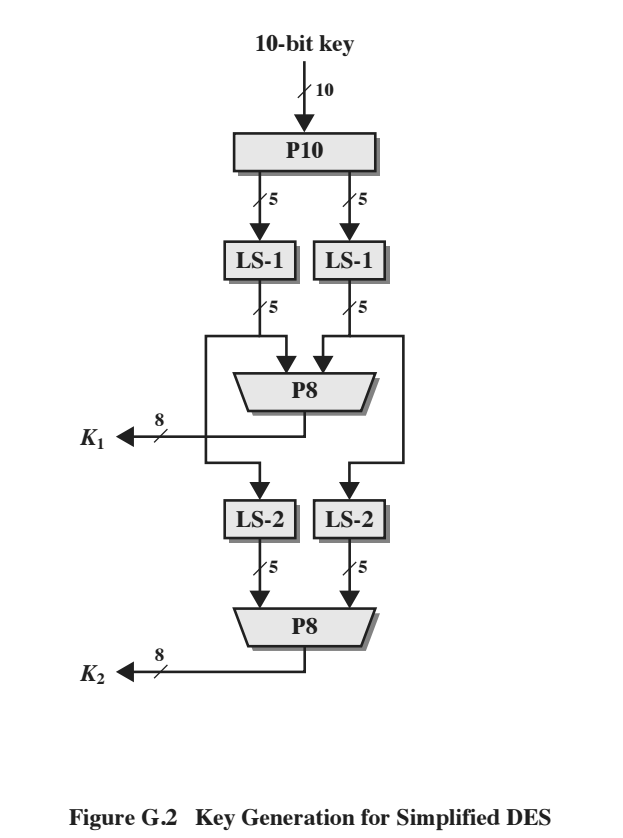
\includegraphics[width=\linewidth]{g2}
  \caption{Figure G.2}
\end{figure}

\subsubsection*{a. How important is the initial P10 permutation function?}
\subsubsection*{b. How important are the two LS-1 shift functions?}

\subsection*{6. (3.17) The equations for the variables q and r for S-DES are
defined in the section on S-DES analysis. Provide the equations for s and t.}

\subsection*{7. (3.18) Using S-DES, decrypt the string (10100010) using the key
(0111111101) by hand. Show intermediate results after each function (IP, F\textsubscript{K}
,SW, F\textsubscript{K} , IP\textsuperscript{-1}). Then decode the first 4 bits of the
plaintext string to a letter and the second 4 bits to another letter where we
encode A through P in base 2 (i.e., A = 0000, B = 0001, ..., P = 1111). Hint: As
a midway check, after the application of SW, the string should be (00010011).}

Geração das subchaves:
\begin{itemize}
  \item chave = 0111111101
  \item P10 = 1111110011
  \item Shift = 1111100111
  \item P8 = 01011111
  \item \textbf{K\textsubscript{1} = 01011111}
  \item Shift = 1111111100
  \item P8 = 11111100
  \item \textbf{K\textsubscript{2} = 11111100}
\end{itemize}

Processo de decifrar:
\begin{itemize}
  \item Texto cifrado = 10100010
  \item IP = 00110001
  \item F\textsubscript{K} =
  \begin{itemize}
    \item E/P = 10000010
    \item E/P xor K\textsubscript{1} = 11011101
    \item S0
  \end{itemize}
\end{itemize}
\end{document}
